\documentclass{article}
\usepackage[utf8]{inputenc}
\usepackage{mathrsfs, amsmath, mathbbol, graphicx}
    % mathrsfs = símbolos: lagrangiano
        % \mathscr{L}
    % amsmath = romper ecuaciones en nuevas líneas y centrar
        % \begin{split}
        % \end{split}
    % mathbbol = Para mostrar los conjuntos numéricos
    % graphix = Para insertar imágenes

\title{Producto punto y normas (para vectores, matrices, polinomios y funciones continuas)}
\author{
    Jorge Antonio Gómez García \\
    Emiliano Martín Lugo López \\
    Saud Antonio Morales González}
\date{03 de abril de 2022}

\begin{document}
\maketitle

\section{Introducción: espacios vectoriales}

    Un espacio vectorial es un conjunto no vacío $V$ de objetos, llamados \textbf{vectores}, en el que se han definido dos operaciones: la suma y el producto por un escalar (número real).\footnote{Isabel Pustilnik y Federico Gómez, "Espacios y subespacios vectoriales - Definición, propiedades y ejemplos", Álgebra y Geometría Analítica, 8 de noviembre de 2017, https://aga.frba.utn.edu.ar/espacios-y-subespacios-vectoriales/.}

    Se define matemáticamente como:

    \begin{equation*}
        \mathbb{R}^n=\{ (x_1, x_2, \dotsb, x_1), x_i \in \mathbb{R}, i=1,2,3,\dotsb,n \}
    \end{equation*}

    La \textbf{definición} de dicha suma y producto están sujetas a diez axiomas. Mientras que, para un espacio vectorial $\mathbb{R}^2$, se definen como:
    \begin{itemize}
        \item Suma de dos vectores: \\
            $ {\vec{A} + \vec{B}= (a,b) + (c,d) = (a+c, c+d)} $
                
        \item Producto de un escalar por un vector: \\
            $ {a(u, v) = (au, av), a \in \mathbb{R}} $
                
    \end{itemize}

\section{Definición del producto punto}

    El producto punto, (también llamado producto escalar o producto interno) es el resultado de multiplicar las componentes de dos vectores entre sí. Se define como:

    \begin{quote}
        Sea $u$, $v$ y $w$ vectores en un \textbf{espacio vectorial} y sea c cualquier escalar. Un producto punto en $V$ es una función que asocia un número real $\langle u, v\rangle$ con cada par de vectores $u$ y $v$ que cumplen los axiomas listados más adelante:\footnote{Ron Larson, \textit{Algebra lineal. matemáticas} 4, 7a ed. (Ciudad de México: Cengage learning, 2018), 185.}
    \end{quote}

    Los componentes de un vector (o coordenadas de un vector) son las "proyecciones" de ese vector sobre los ejes del plano cartesiano. Una representación gráfica es la siguiente:

    \begin{figure}[h]
        \centering
        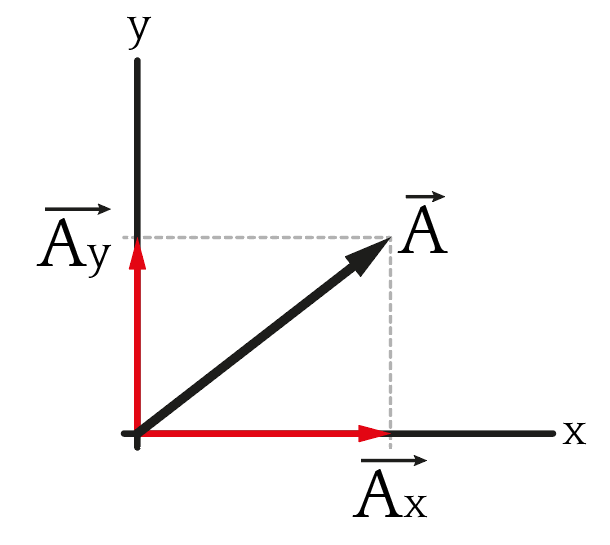
\includegraphics[width=4cm]{img-1-componentes.png}
    \end{figure}

    En este caso el componente horizontal es $\vec{A_x}$, y el componente vertical es $\vec{A_y}$.

    \subsection{Axiomas o propiedades del producto punto}

    \begin{enumerate}

        \item Conmutatividad: \\
            $\langle u, v\rangle = \langle v, u\rangle$
        \item Distributividad con la suma: \\
            $\langle u, v + w\rangle = \langle u, v\rangle + \langle u, w\rangle$
        \item Asociatividad: \\
            $c\langle u, v\rangle=\langle c u, v\rangle=\langle u, c v\rangle$
        \item Propiedad de magnitud: \\
            $\langle v, v\rangle \geq 0$ y $\langle v, v\rangle = 0$ si y sólo si $v = 0$

    \end{enumerate}

    Cuando un espacio vectorial $V$ tiene al menos un producto punto, podemos llamarlo \textbf{espacio con producto punto}. Ahora bien, cuando se hace referencia a un espacio con producto punto, se supone que \textbf{el conjunto de escalares es el conjunto de los números reales}.

    %

\section{Producto punto para vectores}

    Para calcular el producto punto se puede aplicar la siguiente ecuación:

    \begin{equation}
        \vec{A} \cdot \vec{B} = \parallel\vec{A}\parallel \parallel\vec{B}\parallel \cos \theta
    \end{equation}

    Recuerde que $\parallel\vec{A}\parallel$ y $\parallel\vec{B}\parallel$ son las \textbf{magnitudes} o módulos de los vectores $\vec{A}$ y $\vec{B}$.

    Esta es una forma particularmente buena de obtener el producto punto en función del ángulo interno $\theta$ que separa a los dos vectores. Sin embargo la definición del producto punto para $\mathbb{R^2}$ es:

    \begin{equation}
        \vec{A} \cdot \vec{B} = A_xB_x + A_yB_y
    \end{equation}

    Tanto la ecuación $(1)$ como la ecuación $(2)$, son iguales. La primera es un teorema\footnote{Es una interpretación del teorema del coseno} derivado de aplicar la definición del producto punto (la segunda).

    Por lo tanto, tenemos: 
    \begin{equation}
        \vec{A} \cdot \vec{B} = \parallel\vec{A}\parallel \parallel\vec{B}\parallel \cos \theta = A_xB_x + A_yB_y
    \end{equation}
    
    \subsection{Ortogonalidad}
    
        En la ecuación $(3)$, note que si el ángulo interno entre ambos vectores es de 90°, tenemos que $cos \theta = 0$ y, por lo tanto, el produto escalar es igual a $0$. A este tipo de vectores se les llama \textbf{vectores ortogonales}.

        \subsubsection*{Ejemplo:}

            Determinar si los siguientes vectores son ortogonales entre sí:
            \begin{gather*}
                \vec{v}=(2,-3,1) \hspace{35pt} \vec{u}=(3,2,0)
            \end{gather*}

            Calculando el producto punto tenemos que:

            \begin{equation*}
                \begin{aligned}
                    \vec{v} \cdot \vec{u} &=(2,-3,1) \cdot(3,2,0) \\
                    &=(2)(3)+(-3)(2)+(1)(0) \\
                    &=6-6+0 \\
                    &=0
                \end{aligned}
            \end{equation*}

            Al ser el producto punto igual a cero, tenemos dos vectores que son ortogonales entre sí.
    
    \subsection{Módulo de un vector en términos del producto punto (norma)}

        Recuerde que algunos párrafos atrás establecimos que el producto punto es el resultado de multiplicar las magnitudes de los vectores por el coseno de $\theta$. Pues bien, la magnitud (también llamada módulo o norma) de un vector $\vec{A}$ se escribe $\parallel\vec{A}\parallel$ y se \textbf{define} como:

        \begin{align}
            \parallel \vec{A}\parallel &= \sqrt{\langle \vec{A}, \vec{A}\rangle} = \sqrt{\vec{A} \cdot \vec{A}} = \sqrt{A_{1}^{2}+A_{2}^{2}+\cdots+A_{n}^{2}}
        \end{align}

        Esto quiere decir que la norma de un vector es la raíz de la suma de los componentes del vector multiplicados consigo mismos.

        Algunas propiedades de la norma de un vector son las siguientes:

        \begin{itemize}

            \item La norma de $\vec{A}$ es $\parallel \vec{A}\parallel$ = $\sqrt{\vec{A} \cdot \vec{A}}$
            \item La distancia entre $\vec{A}$ y $\vec{B}$ es $d(\vec{A}, \vec{B}) = \parallel \vec{A} - \vec{B} \parallel$
            \item El ángulo entre dos vectores diferentes de cero $\vec{A}$ y $\vec{B}$ está determinado por: \\
            \begin{equation}
                \cos \theta=\frac{\langle\vec{A}, \vec{B}\rangle}{\parallel\vec{A}\parallel\parallel\vec{B}\parallel}, \quad 0 \leq \theta \leq \pi
            \end{equation}
            \item Si $\langle \vec{A}, \vec{B}\rangle = 0$, $\vec{A}$ y $\vec{B}$ son ortogonales entre sí.

        \end{itemize}

        \subsubsection*{Ejemplo:}

        Determinar la norma del siguiente vector:

        \begin{equation*}
            \vec{v}=(-3,2,5)
        \end{equation*}

        Para ello:

        \begin{equation*}
            \begin{aligned}
            \parallel \vec{v}\parallel &=\sqrt{\vec{v} \cdot \vec{v}} \\
            &=\sqrt{(-3,2,5) \cdot(-3,2,5)} \\
            &=\sqrt{(-3)^{2}+(2)^{2}+(5)^{2}} \\
            &=\sqrt{9+4+25} \\
            &=\sqrt{38}
            \end{aligned}
        \end{equation*}

    \subsection{Ángulo entre dos vectores en términos de su producto punto}

        Al igual que la norma y la condición de ortogonalidad, el producto punto sirve para determinar el ángulo de separación entre dos vectores. Para determinar el ángulo interior entre dos vectores $\vec{A}$ y $\vec{B}$ en términos de su producto punto, necesitamos determinar el coseno de su ángulo ($\theta$).

        Para obtener dicho coseno se cumple que:

        \begin{equation}
            \cos \theta = \frac{\vec{A} \cdot \vec{B}}{\parallel\vec{A}\parallel\parallel\vec{B}\parallel} = \frac{A_{1} B_{1}+A_{1} B_{1}+\cdot+A_{n} B_{n}}{\sqrt{A_{1}^{2}+A_{2}^{2}+\cdots+A_{n}^{2}} \sqrt{B_{1}^{2}+B_{2}^{2}+\cdots+B_{n}^{2}}}
        \end{equation}

        Una vez que ha determinado el valor del coseno de $\theta$, puede aplicar la función trigonométrica inversa para conocer el ángulo de separación entre $\vec{A}$ y $\vec{B}$:

        \begin{equation}
            \theta=\arccos \left(\frac{\vec{A} \cdot \vec{B}}{|\vec{A}||\vec{B}|}\right)
        \end{equation}

        \subsubsection*{Ejemplo:}

            A partir del siguiente par de vectores, determine el ángulo de separación entre el vector $\vec{A}$ y el  $\vec{B}$:

            \begin{gather*}
                \vec{A}=(1,2,-3) \hspace*{35 pt} \vec{B}=(-2,4,1)
            \end{gather*}
        
            Solución:

            \begin{equation}
                \begin{aligned}
                \theta &=\arccos \left(\frac{\vec{A} \cdot \vec{B}}{|\vec{A}||\vec{B}|}\right) \\
                &=\arccos \left(\frac{(1)(-2)+(2)(4)+(-3)(1)}{\sqrt{(1)^{2}+(2)^{2}+(-3)^{2}} \sqrt{(-2)^{2}+(4)^{2}+(1)^{2}}}\right) \\
                &=\arccos \left(\frac{-2+8+-3}{\sqrt{1+4+9} \sqrt{4+16+1}}\right) \\
                &=\arccos \left(\frac{3}{\sqrt{14} \sqrt{21}}\right) \\
                &=\arccos \left(\frac{3}{\sqrt{(7)(2)} \sqrt{(7)(3)}}\right) \\
                &=\arccos \left(\frac{3}{\sqrt{(7)^{2}(2)(3)}}\right) \\
                &=\arccos \left(\frac{3}{7 \sqrt{6}}\right) \\
                &=79.92^{\circ}
                \end{aligned}
            \end{equation}

\section{Producto punto para matrices}

    Las propiedades de la multiplicación de matrices son causa directa de muchas de las propiedades del producto punto. También se puede obtener el producto punto de la multiplicación de matrices. Para ello, se sigue el siguiente procedimiento:

    Definiendo a $A$ y $B$ como matrices pertenecientes a un espacio vectorial $M$, donde:

    \begin{gather}
        A = \begin{bmatrix}
           a_{11} & a_{12} \\
           a_{21} & a_{22}
        \end{bmatrix} \hspace{35 pt}
        B = \begin{bmatrix}
            b_{11} & b_{12} \\
            b_{21} & b_{22}
        \end{bmatrix}
    \end{gather}

    tenemos que:

    \begin{equation}
        \langle A, B\rangle=a_{11} b_{11}+a_{21} b_{21}+a_{12} b_{12}+a_{22} b_{22}
    \end{equation}

    es un producto punto de $A$ y $B$ sobre el espacio vectorial $M$.

    En adición, los vectores pueden ser representados en matrices en una forma de matriz columna de $n\times1$. De tal forma que un vector $u = (u_1, u_2, \cdots, u_n)$ donde $u \in \mathbb{R}$ puede representarse de forma matricial como:

    \begin{equation}
        u=\left[\begin{array}{c}
        u_{1} \\
        u_{2} \\
        \vdots \\
        u_{n}
        \end{array}\right]
    \end{equation}

    Ahora bien, si tenemos otra matriz $v$, definida como:

    \begin{equation}
        v=\left[\begin{array}{c}
        v_{1}  \\
        v_{2}  \\
        \vdots \\
        v_{n}
        \end{array}\right]
    \end{equation}

    y deseamos obtener el producto punto de ambas matrices, tenemos que:

    \begin{equation}
        \begin{aligned}
            u \cdot v=u^{T} v &= \left[\begin{array}{llll}
            u_{1} & u_{2} & \ldots & u_{n}
            \end{array}\right]\left[\begin{array}{c}
            v_{1} \\
            v_{2} \\
            \vdots \\
            v_{n}
            \end{array}\right] \\ &= \left[u_{1} v_{1}+u_{2} v_{2}+\cdots+u_{n} v_{n}\right]
        \end{aligned}
    \end{equation}

    \subsubsection*{Ejemplo:}

    Determine el producto punto de las siguientes matrices:

    \begin{gather*}
        A = \begin{bmatrix}
            1  \\
            4  \\
            -6
        \end{bmatrix} \hspace{35 pt}
        B = \begin{bmatrix}
            4  \\
            -2 \\
            -1
        \end{bmatrix}
    \end{gather*}

    Solución usando la ecuación $(13)$:

    \begin{equation*}
        \begin{aligned}
            A \cdot B = A^TB = \begin{bmatrix}
                1 & 4 & -6
            \end{bmatrix} \begin{bmatrix}
                4 \\
                -2 \\
                -1
            \end{bmatrix}
            &=[(1)(4) + (4)(-2) + (-6)(-1)] \\
            &=4-8+6 \\
            &=2
        \end{aligned}
    \end{equation*}

    Como resultado de multiplicar $A \cdot B$, tenemos un producto punto de $2$.

\section{Producto punto para polinomios}

   No necesariamente todas las funciones son producto punto. Para que pueda considerarse un producto punto en $R^n$ es necesario que se cumplan los cuatro axiomas que definen al producto punto.

   \subsubsection*{Ejemplo:}

    Para desarrollar algunos ejemplos de producto punto sobre polinomios considere los siguientes polinomios:
    \begin{gather*}
        p(x)=1-2x^{2}\hspace{35pt}q(x)=4-2x+x^{2}\hspace{35pt}r(x)=x+2x^{2}
    \end{gather*}

    Determine:
    \begin{gather*}
        \textbf{a.}\hspace{2pt}\langle p,q\rangle\hspace{30pt}\textbf{b.}\hspace{2pt}\langle q,r\rangle\hspace{30pt}\textbf{c.}\hspace{2pt}\parallel q\parallel\hspace{35pt}\textbf{d.}\hspace{2pt}d(p,q)
    \end{gather*}

    \textbf{a.}
        \begin{align*}
            \langle p,q\rangle&= (4)(1)+(0)(-2)+(-2)(1) & \\
            \langle p,q\rangle&= 4+0-2 & \\
            \langle p,q\rangle&= 2
        \end{align*}

    \textbf{b.}
        \begin{align*}
            \langle q,r\rangle&= (4)(0)+(-2)(1)+(1)(2) & \\
            \langle q,r\rangle&= 0-2+2 & \\
            \langle q,r\rangle&= 0
        \end{align*}

    \textbf{c.}
        \begin{align*}
            \parallel p\parallel&= \sqrt{\langle q,q\rangle} & \\
            \parallel p\parallel&= \sqrt{(4)(4)+(-2)(-2)+(1)(1)} \\
            \parallel p\parallel&=\sqrt{4^{2}+(-2)^{2}+1^{2}} & \\
            \parallel p\parallel&= \sqrt{16+4+1} & \\
            \parallel p\parallel&= \sqrt{21}
        \end{align*}

    \textbf{d.}
        \begin{align*}
            d(p,q)&= \parallel p-q\parallel & \\
            d(p,q)&= \parallel (1-2x^{2})-(4-2x+x^{2})\parallel & \\
            d(p,q)&= \parallel -3+2x-3x^{2}\parallel & \\
            d(p,q)&= \sqrt{(-3)^{2}+2^{2}+(-3)^{2}} & \\
            d(p,q)&= \sqrt{22}
        \end{align*}

\section{Producto punto para funciones continuas}

    El producto punto en una función continua se puede determinar por medio de una integral definida.

    Sean $f$ y $g$ funciones continuas de valores reales en el espacio vectorial $C[a, b]$, la siguiente operación define un producto punto:

    \begin{equation}
        \langle f, g\rangle=\int_{a}^{b} f(x) g(x) d x
    \end{equation}

\section{Tarea}

    Para desarrollar sus habilidades, practique con los siguientes ejercicios:

    \subsection{Producto punto para vectores}

        \subsubsection{Ortogonalidad}

            Determine si los siguientes dos vectores son ortogonales:
            \begin{gather*}
                \vec{A} = (6,2,4) \hspace*{35 pt} \vec{B}=(2,4,0)
            \end{gather*}

        \subsubsection{Norma de un vector}

            Determine la norma del siguiente vector:
            \begin{gather*}
                \vec{A} = (6,4,-7,2)
            \end{gather*}

        \subsubsection{Ángulo entre dos vectores}

            Determine el ángulo entre el vector $\vec{A}$ y el vector $\vec{B}$:
            \begin{gather*}
                \vec{A} = (6,-2,-4) \hspace*{35 pt} \vec{B} = (0, 3, -7)
            \end{gather*}

    \subsection{Producto punto para matrices}

            Sean la matriz $A$ y $B$ pertenecientes al espacio vectorial $M$, determine el producto punto:
            \begin{gather*}
                A = \begin{bmatrix}
                    3  & 7 \\
                    -4 & 1
                \end{bmatrix} \hspace*{35 pt}
                B = \begin{bmatrix}
                    -6 & -2 \\
                    4  & 7
                \end{bmatrix}
            \end{gather*}
    
    \subsection{Producto punto para polinomios}

        Determine el producto punto de los siguientes polinomios:
        \begin{gather*}
            f(x) = 3x^3 - 6x^2 + 4x + 3 \hspace*{35 pt}
            g(x) = 4x^3 + 3x - 7
        \end{gather*}

\pagebreak
    
\section*{Bibliografía}
    
    \paragraph{El Traductor de Ingeniería. "Vectores: ¿Flechas o Espacios Vectoriales?... ¿o ambos?" YouTube, 12 de diciembre de 2021. Video, 58:21. https://www.youtube.com/watch?v=eXA4806YuqY.}
    
    \paragraph{Larson, Ron. Algebra lineal. matemáticas 4. 7a ed. Ciudad de México: Cengage learning, 2018.}
    
    \paragraph{Pustilnik, Isabel y Federico Gómez. "Espacios y subespacios vectoriales - Definición, propiedades y ejemplos". Álgebra y Geometría Analítica, 8 de noviembre de 2017. https://aga.frba.utn.edu.ar/espacios-y-subespacios-vectoriales/.}
    
    \paragraph{Superprof. "Producto punto". Material Didáctico - Superprof, 2020. https://www.superprof.es/apuntes/escolar/matematicas/analitica/\\
    vectores/producto-punto.html}
    
\end{document}
